% !TeX root = ../../main.tex
\subsection{Servidor DNS e Nginx}

Após a configuração dos serviços DNS e Nginx, foi realizado um teste de acesso ao servidor web utilizando o nome de domínio previamente configurado no servidor DNS. O objetivo foi validar tanto a resolução de nomes quanto a disponibilidade do serviço HTTP hospedado na rede DMZ.

Conforme apresentado na Figura \ref{fig:nginx}, o cliente acessou o endereço \texttt{web.conectanet.local} por meio do navegador Firefox, sem a necessidade de informar diretamente o endereço IP do servidor. A correta exibição da página demonstra que o serviço DNS realizou a resolução do nome para o endereço IP correspondente e que o servidor Nginx respondeu adequadamente à requisição HTTP.

Os resultados obtidos confirmam o funcionamento integrado dos serviços DNS e Nginx, evidenciando que o ambiente foi configurado corretamente e que os clientes da rede conseguem acessar o servidor web utilizando nomes de domínio, proporcionando maior facilidade de utilização e administração da infraestrutura.

\begin{figure}[H]
    \centering
    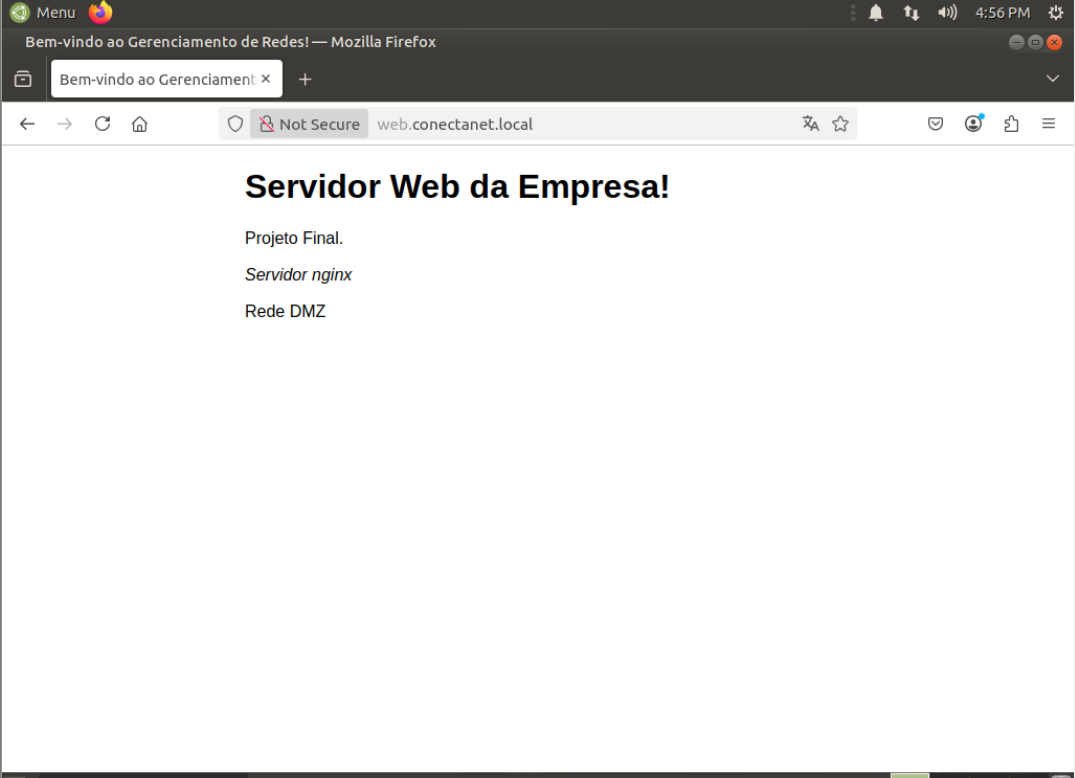
\includegraphics[width=1\linewidth]{fig/nginx.png}
    \caption{Acesso ao servidor web utilizando a resolução de nomes fornecida pelo servidor DNS.}
    \label{fig:nginx}
\end{figure}


\subsection{Serviço SFTP}

Após a configuração do serviço SFTP, foram realizados testes de transferência de arquivos entre o cliente e o servidor para validar seu funcionamento. A autenticação foi realizada utilizando credenciais previamente cadastradas no servidor, estabelecendo uma conexão segura por meio do protocolo SSH.

Durante os testes foram executadas operações de envio e recebimento de arquivos e diretórios, utilizando os principais comandos disponibilizados pelo cliente SFTP:

\begin{itemize}
    \item Enviar um arquivo:
    \begin{center}
        \texttt{put teste.txt}
    \end{center}

    \item Enviar um diretório:
    \begin{center}
        \texttt{put -r Documentos}
    \end{center}

    \item Baixar um arquivo:
    \begin{center}
        \texttt{get relatorio.pdf}
    \end{center}

    \item Baixar um diretório:
    \begin{center}
        \texttt{get -r backup}
    \end{center}
\end{itemize}

A Figura \ref{fig:sftp} apresenta um dos testes realizados, no qual é estabelecida a conexão com o servidor SFTP e executado o comando \texttt{get -r dialog}, responsável por realizar o download recursivo do diretório \texttt{dialog}. A saída exibida confirma a transferência dos arquivos presentes no diretório, indicando o progresso da cópia e as respectivas taxas de transferência.

Os resultados obtidos demonstram o funcionamento adequado do serviço SFTP, possibilitando a transferência segura de arquivos e diretórios entre cliente e servidor por meio da porta TCP 22, garantindo confidencialidade dos dados durante a comunicação.

\begin{figure}[H]
    \centering
    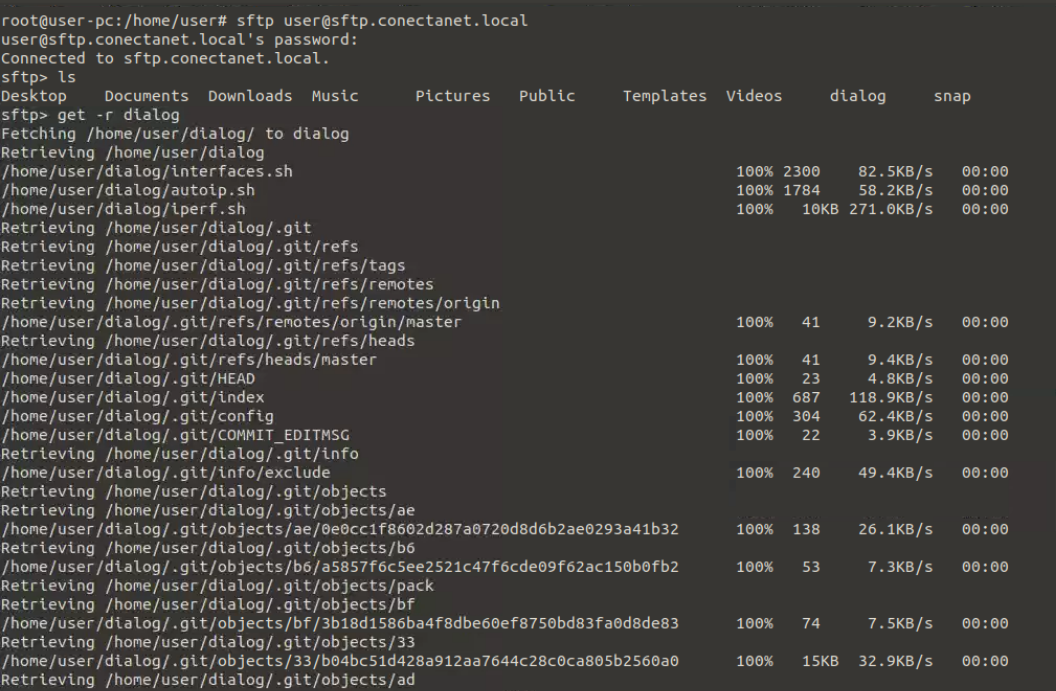
\includegraphics[width=1\linewidth]{fig/sftp.png}
    \caption{Transferência de diretório utilizando o serviço SFTP.}
    \label{fig:sftp}
\end{figure}


\subsection{Servidor Samba}

Após a configuração do servidor Samba na máquina virtual Linux, foi realizado um teste de acesso a partir do computador Windows. O compartilhamento foi acessado por meio do Explorador de Arquivos utilizando o endereço IP do servidor, demonstrando a correta integração entre os sistemas Linux e Windows.

Conforme apresentado na Figura \ref{fig:samba}, o diretório compartilhado foi identificado e acessado com sucesso pelo cliente Windows, sendo possível visualizar a pasta disponibilizada pelo servidor. Esse resultado confirma o funcionamento adequado do serviço Samba, bem como a conectividade entre os dispositivos da rede e as permissões de compartilhamento configuradas.

\begin{figure}[H]
    \centering
    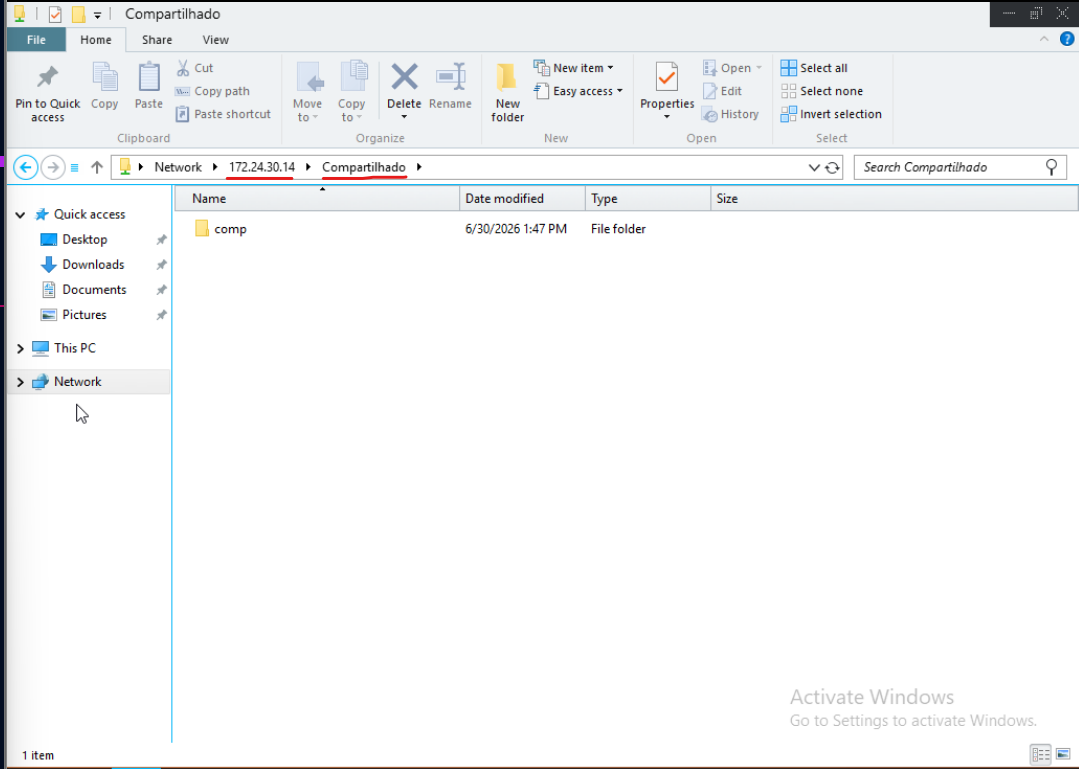
\includegraphics[width=1\linewidth]{fig/samba.png}
    \caption{Acesso ao diretório compartilhado no servidor Samba a partir do Windows.}
    \label{fig:samba}
\end{figure}

